\namedsection{ARM Cortex M0+Processor}{Pasat}

This section discusses one of the main requirement and one of the essential aspect of our project, ARM’s Cortex M0 processor. This processor is the member of the Cortex-M family in term of costs and performance/functionality. It has been designed in order to allow intelligent compromises in terms of power usage, computational power and in the simplicity of the design. It implements a simplified version of the Advanced Microcontroller Bus Architecture (AMBA), the AMBA-Lite bus which allows connection to different peripherals. In this way, the Cortex-M0 generally acts as the master device and the peripherals act as slaves. Below, in figure \ref{fig:cortexm0ds}, the schematic for the processor can be seen.\\
\begin{figure}
\centering
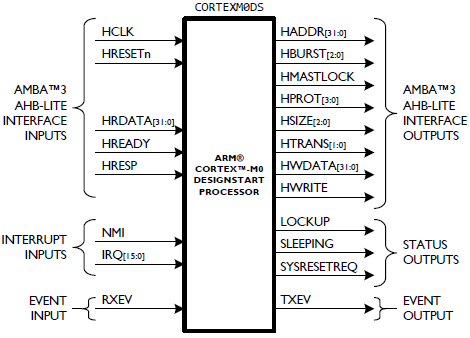
\includegraphics[scale=0.7]{figures/cortexm0ds_schematic.PNG}
\caption{Cortex M0DS schematic \label{fig:cortexm0ds}}
\end{figure}
\clearpage

\begin{figure}
\centering
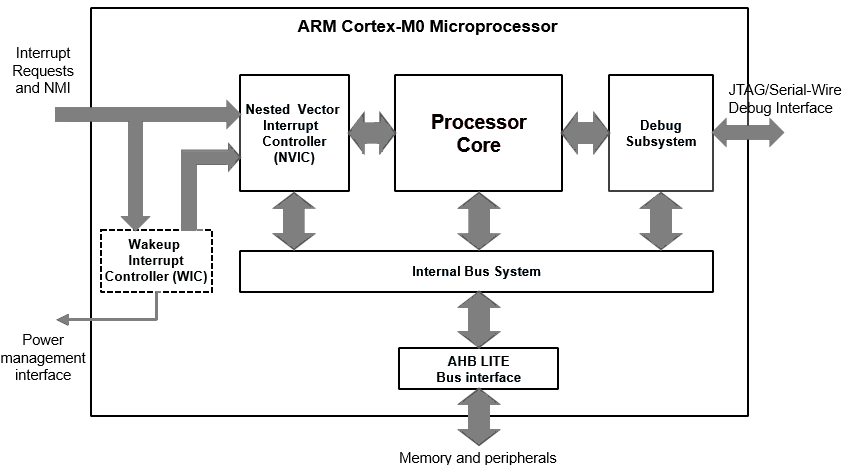
\includegraphics[scale=0.7]{figures/arm_cortexm0_microprocessor.PNG}
\caption{Cortex M0DS schematic \label{fig:cortex_block}}
\end{figure}

The Cortex M0+ has a 32-bit reduced instruction set computing(RISC) processor. It uses the ARMv6-M(which stands for Microcontroller), which is a subset of the ARMv7-M profile but it includes fewer instructions. The Cortex M0 is based on a Von-Neumann architecture, having both data and instructions share a single bus interface. It provides a Debug Extension that includes some architectural extensions to support debugging. The ARMv6-M offers support for 56 as a subset of  Thumb-1(16-bit) and Thumb-2(16/32b-bit) which are present in the ARMv6T2. The Cortex M0+ block diagram can be seen above in figure \ref{fig:cortex_block}. 

The Processor Core contains the internal registers, data path, ALU and control logics. The Cortex M0 has a three-stage pipeline: fetch, decode and exection and includes the 32-bit registers for general and special usages. The Cortex M0+ has only a two-stage pipeline to reduce the power usage.

The Nested Vectored Interrupt Controller(NVIC) handles up to 32 interrupts request signals and one NMI(shortcut in list of symbols) . It also fulfils tasks such as comparing priorities between  interrupt requests and the current priority level. 

The Bus system contains the internal bus system, data path in the processor core and the AHB LITE interface unit which is an on-chip bus protocol which enables some features required for high-performance, high clock frequency systems. 

The Debug system handles the program breakpoints, debugging control and the data watchpoints. This can put the processor in a  static state in order for the programmer to evaluate and analyse the status of the processor in that specific moment.

The Wakeup Interrupt Controller (WIC) is important for this project because it is used in low-power applications. The microcontroller can be set to enter sleep mode by turning off most of it's components. If a interrupt request is sent, this component can inform the unit that handles the power management to power up the system.

One of the major challenges which were encountered in the use of the Cortex M0+ is the absence of the hardware dividing unit and floating point  on the device. This was mitigated by scaling each double value by $2^{12}$ and taking the integer part. After each multiplication, the value is bit-shifted by 12 to keep the scale factor consistent. This was described earlier in more detail in the software section.

Through the aid of our client, ARM, we managed to gain access to a fixed configuration of the Cortex-M0 Processor know as Cortex-M0 DesignStart. This simplified version offers us access to a Verilog version of the Cortex-M0 under the form of an obfuscated and preconfigured netlist, but it can be synthesized. This package offers us some Verilog code and a test-bench which allow a simulation of the Cortex-M0 DesignStart module connected to a memory model and a clock and reset generator. Also, access was given to the CM0DS example design kit which contains various AHB-Lite peripherals and infrastructure components, useful to create complete systems. Before implementing the actual algorithm on the FPGA, a more basic simulation needs to be conducted on the platform to assure that it is compatible with the specific FPGA used. In the following sections we will discuss about the mBed platform which contains the Cortex M0+ and the Digilent Nexys4 FPGA board on which we aimed to implement the microprocessor as an extension.
